\documentclass[12pt]{article}
\usepackage{amsmath}
\usepackage{listings}
\usepackage{color}
\usepackage{geometry}
\usepackage{float} % Required for the [H] float option
\usepackage{graphicx} % Required for including images
\geometry{margin=1in}
\usepackage{caption}
\usepackage[colorlinks=true, linkcolor=black, urlcolor=blue, citecolor=blue]{hyperref}
\usepackage{fancyhdr}
\usepackage{color}
\usepackage{xcolor} % Needed for custom colors
\definecolor{purple}{rgb}{0.5,0.0,0.5} % Define purple manually
\definecolor{codegray}{rgb}{0.5,0.5,0.5}
\definecolor{backcolour}{rgb}{0.95,0.95,0.92}




\pagestyle{fancy}
\fancyhead[L]{ Assignment -3 }
\fancyhead[R]{Gandholi Sarat - 23008}
\title{\textbf{PMAT 402 - Systems Programming \\ Assignment -3 \\ Simplified Pascal Compiler in C++}}
\author{\textbf{Gandholi Sarat - 23008}}
\author{Gandholi Sarat - 23008}
\date{April 10, 2025}

\definecolor{codegray}{rgb}{0.5,0.5,0.5}
\definecolor{backcolour}{rgb}{0.95,0.95,0.92}
\lstdefinestyle{mystyle}{
    backgroundcolor=\color{backcolour},   
    commentstyle=\color{codegray},
    keywordstyle=\color{blue},
    numberstyle=\tiny\color{codegray},
    stringstyle=\color{purple},
    basicstyle=\ttfamily\footnotesize,
    breakatwhitespace=false,         
    breaklines=true,                 
    captionpos=b,                    
    keepspaces=true,                 
    numbers=left,                    
    numbersep=5pt,                  
    showspaces=false,                
    showstringspaces=false,
    showtabs=false,                  
    tabsize=2
}
\lstset{style=mystyle}

\begin{document}


\maketitle
\tableofcontents
\newpage

\section{Objective}
To design and implement (as an entire class of students) a recursive descent parser in C++
for a simple programming language resembling Pascal, incorporating lexical analysis, syntax
rules, and parsing functions to validate program input.

\section{Pascal Grammar Given}

\begin{figure}[H]
\centering
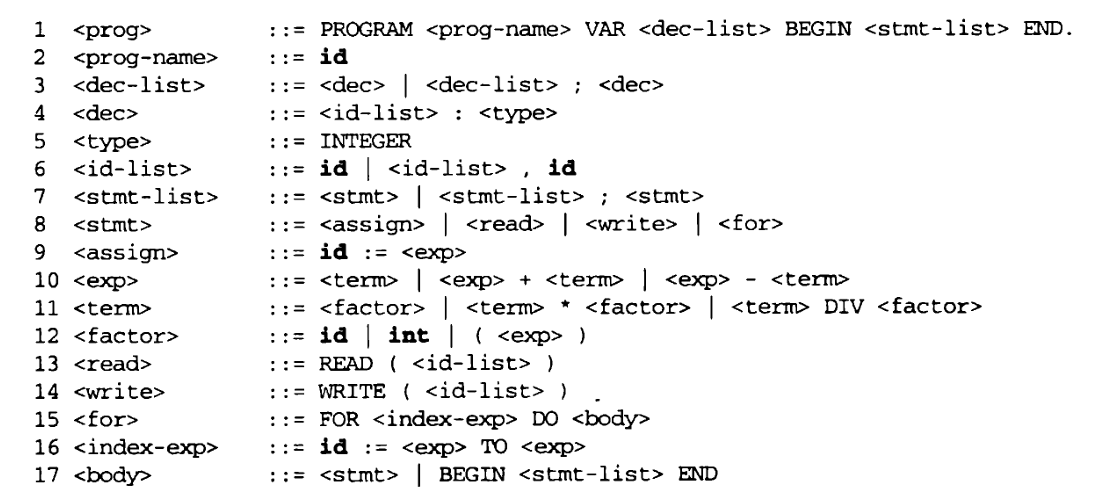
\includegraphics[width=\textwidth]{Pascal.png}
\caption{Pascal Grammar}
\label{fig:grammar}
\end{figure}

\section{Code Explanation}

\subsection{Lexical Mapping}
The lex map defines token-to-integer associations for keywords, symbols, and identifiers. This simulates the output of a lexical analyzer.

\begin{lstlisting}[language=C++]
map <string , int > lex = {
  {"PROGRAM", 1}, {"VAR", 2}, {"BEGIN", 3}, ..., {"int", 23}
};
\end{lstlisting}

\subsection{Tokenization}
The tokenize function splits the input string into words and converts them into token integers using the lex map. If an unknown token is encountered, an error is displayed and the program exits.

\subsection{Token Management}
The current token is managed using a global variable TOKEN, and the function \texttt{get\_NextToken()} retrieves the next token from the token stream.

\begin{lstlisting}[language=C++]
int get_NextToken () {
  if (index1 < tokens.size()) {
    return tokens[index1++];
  }
  return -1;
}
\end{lstlisting}

\subsection{Parsing Functions}
Each function corresponds to a non-terminal symbol in the grammar. These functions recursively validate the input token sequence.

\begin{itemize}
  \item \texttt{prog()} parses the full program structure.
  \item \texttt{stmt()} identifies whether a statement is an assignment, read, write, or for-loop.
  \item \texttt{exp()}, \texttt{term()}, and \texttt{factor()} handle expressions based on operator precedence.
\end{itemize}

Example: \texttt{assign()} checks if a statement is in the form \texttt{i := expression}:

\begin{lstlisting}[language=C++]
bool assign () {
  if (TOKEN == 22) {
    TOKEN = get_NextToken ();
    if (TOKEN == 15) {
      TOKEN = get_NextToken ();
      if (exp()) {
        return true;
      }
    }
  }
  return false;
}
\end{lstlisting}

\subsection{Parsing Entry Point}
The \texttt{parse()} function serves as the entry point for the parser. It first tokenizes the input string and initializes the token stream. The syntax validation process begins by invoking \texttt{stmt()}, which acts as the top-level non-terminal for parsing single or compound statements. If the entire token stream is successfully consumed and validated, the input is deemed syntactically correct; otherwise, an error message is displayed.

\begin{lstlisting}[language=C++]
void parse(string input) {
  tokens = tokenize(input);
  index1 = 0;
  TOKEN = get_NextToken ();
  if (stmt() && index1 == tokens.size()) {
    cout << "Valid syntax\n";
  } else {
    cout << "Invalid syntax\n";
  }
}
\end{lstlisting}

\subsection{Main Function}
The \texttt{main()} function reads user input and passes it to \texttt{parse()} for validation.
\begin{lstlisting}[language=C++]
int main() {
  string input;
  cout << "Enter input string: ";
  getline(cin, input);
  parse(input);
  return 0;
}
\end{lstlisting}

\section{Full Code}
\begin{lstlisting}[language=C++]
  #include <iostream>
  #include <string>
  #include <map>
  #include <sstream>
  #include <vector>
  
  using namespace std;
  
  map<string, int> lex = {
      {"PROGRAM", 1}, {"VAR", 2}, {"BEGIN", 3}, {"END", 4}, {"END.", 5},
      {"INTEGER", 6}, {"FOR", 7}, {"READ", 8}, {"WRITE", 9}, {"TO", 10},
      {"DO", 11}, {";", 12}, {":", 13}, {",", 14}, {":=", 15},
      {"+", 16}, {"-", 17}, {"*", 18}, {"DIV", 19}, {"(", 20}, {")", 21},
      {"i", 22}, {"int", 23}
  };
  
  vector<int> tokens;
  int index1 = 0;
  int TOKEN = -1;
  
  vector<int> tokenize(string input) {
      vector<int> tokenList;
      stringstream ss(input);
      string word;
      while (ss >> word) {
          if (lex.find(word) != lex.end()) {
              tokenList.push_back(lex[word]);
          } else {
              cout << "Error: Unknown token '" << word << "'\n";
              exit(1);
          }
      }
      return tokenList;
  }
  
  int get_NextToken() {
      if (index1 < tokens.size()) {
          return tokens[index1++];
      }
      return -1;
  }
  
  bool prog();
  bool prog_name();
  bool dec_list();
  bool type();
  bool id_list();
  bool stmt_list();
  bool stmt();
  bool assign();
  bool exp();
  bool term();
  bool factor();
  bool read();
  bool write();
  bool for_stmt();
  bool index_exp();
  bool body();
  
  bool prog() {
      if (TOKEN == 1) { // PROGRAM
          TOKEN = get_NextToken();
          if (prog_name()) {
              if (TOKEN == 2) { // VAR
                  TOKEN = get_NextToken();
                  if (dec_list()) {
                      if (TOKEN == 3) { // BEGIN
                          TOKEN = get_NextToken();
                          if (stmt_list()) {
                              if (TOKEN == 4) { // END
                                  TOKEN = get_NextToken();
                                  if (TOKEN == 5) { // END.
                                      TOKEN = get_NextToken();
                                      return index1 == tokens.size();
                                  }
                              }
                          }
                      }
                  }
              }
          }
      }
      return false;
  }
  
  bool prog_name() {
      return TOKEN == 22; // i
  }
  
  bool dec_list() {
      if (id_list()) {
          if (TOKEN == 13) { // :
              TOKEN = get_NextToken();
              if (type()) {
                  return true;
              }
          }
      }
      return false;
  }
  
  bool type() {
      return TOKEN == 6; // INTEGER
  }
  
  bool id_list() {
      if (TOKEN == 22) { // i
          TOKEN = get_NextToken();
          while (TOKEN == 14) { // ,
              TOKEN = get_NextToken();
              if (TOKEN != 22) return false;
              TOKEN = get_NextToken();
          }
          return true;
      }
      return false;
  }
  
  bool stmt_list() {
      if (stmt()) {
          while (TOKEN == 12) { // ;
              TOKEN = get_NextToken();
              if (!stmt()) return false;
          }
          return true;
      }
      return false;
  }
  
  bool stmt() {
      return assign() || read() || write() || for_stmt();
  }
  
  bool assign() {
      if (TOKEN == 22) { // i
          TOKEN = get_NextToken();
          if (TOKEN == 15) { // :=
              TOKEN = get_NextToken();
              if (exp()) {
                  return true;
              }
          }
      }
      return false;
  }
  
  bool exp() {
      if (term()) {
          while (TOKEN == 16 || TOKEN == 17) { // + or -
              TOKEN = get_NextToken();
              if (!term()) return false;
          }
          return true;
      }
      return false;
  }
  
  bool term() {
      if (factor()) {
          while (TOKEN == 18 || TOKEN == 19) { // * or DIV
              TOKEN = get_NextToken();
              if (!factor()) return false;
          }
          return true;
      }
      return false;
  }
  
  bool factor() {
      if (TOKEN == 22 || TOKEN == 23) { // i or int
          TOKEN = get_NextToken();
          return true;
      } else if (TOKEN == 20) { // (
          TOKEN = get_NextToken();
          if (exp()) {
              if (TOKEN == 21) { // )
                  TOKEN = get_NextToken();
                  return true;
              }
          }
      }
      return false;
  }
  
  bool read() {
      if (TOKEN == 8) { // READ
          TOKEN = get_NextToken();
          if (TOKEN == 20) { // (
              TOKEN = get_NextToken();
              if (id_list()) {
                  if (TOKEN == 21) { // )
                      TOKEN = get_NextToken();
                      return true;
                  }
              }
          }
      }
      return false;
  }
  
  bool write() {
      if (TOKEN == 9) { // WRITE
          TOKEN = get_NextToken();
          if (TOKEN == 20) { // (
              TOKEN = get_NextToken();
              if (id_list()) {
                  if (TOKEN == 21) { // )
                      TOKEN = get_NextToken();
                      return true;
                  }
              }
          }
      }
      return false;
  }
  
  bool for_stmt() {
      if (TOKEN == 7) { // FOR
          TOKEN = get_NextToken();
          if (index_exp()) {
              if (TOKEN == 10) { // TO
                  TOKEN = get_NextToken();
                  if (exp()) {
                      if (TOKEN == 11) { // DO
                          TOKEN = get_NextToken();
                          if (body()) {
                              return true;
                          }
                      }
                  }
              }
          }
      }
      return false;
  }
  
  bool index_exp() {
      if (TOKEN == 22) { // i
          TOKEN = get_NextToken();
          if (TOKEN == 15) { // :=
              TOKEN = get_NextToken();
              if (exp()) {
                  return true;
              }
          }
      }
      return false;
  }
  
  bool body() {
      return stmt() || (TOKEN == 3 && stmt_list() && TOKEN == 4); // BEGIN stmt-list END
  }
  
  void parse(string input) {
      tokens = tokenize(input);
      index1 = 0;
      TOKEN = get_NextToken();
      if (stmt() && index1 == tokens.size()) { // Changed from prog() to stmt()
          cout << "Valid syntax\n";
      } else {
          cout << "Invalid syntax\n";
      }
  }
  
  int main() {
      string input;
      cout << "Enter input string: ";
      getline(cin, input);
      parse(input);
      return 0;
  }
\end{lstlisting}

\section{Code Output}
\begin{verbatim}
Enter input string: i := i * i
Valid syntax

Enter input string: i := i DIV i
Valid syntax

Enter input string: READ ( i , i , i )
Valid syntax

Enter input string: WRITE ( i , i )
Valid syntax

Enter input string: i := i DIV
Invalid syntax

Enter input string: WRITE ( i ,
Invalid syntax
\end{verbatim}

\end{document}
